\documentclass[a4paper, 12pt]{article}
\usepackage[utf8]{inputenc}
\renewcommand\familydefault{\sfdefault}
\usepackage[T1]{fontenc}
\usepackage[francais]{babel}
\usepackage[left=2cm,top=2cm,right=2cm,bottom=2cm]{geometry}
\usepackage{graphicx}
\usepackage{minted}
\usemintedstyle{colorful}
\usepackage{float}
\floatplacement{figure}{H}
\usepackage{authblk}
\usepackage{enumitem}
\usepackage{hyperref}
\hypersetup{
	colorlinks,
	citecolor=black,
	filecolor=black,
	linkcolor=black,
	urlcolor=blue
}

\usepackage{caption}
\newenvironment{code}{\captionsetup{type=listing}}{}

\begin{document}

\title{Doge FS}
\author{Raed Abdennadher et Steven Liatti}
\affil{\small Programmation avancée des systèmes - Prof. Florent Glück}
\affil{\small Hepia ITI 3\up{ème} année}
\maketitle

% \begin{figure}
% 	\begin{center}
% 		\includegraphics[width=1.0\textwidth]{intro.png}
% 	\end{center}
% \end{figure}
% \newpage

% \tableofcontents
% \listoffigures
% \renewcommand\listoflistingscaption{Table des listings de code source}
% \listoflistings

% \newpage

\section{Description}
Ce rapport décrit le système de fichiers "Doge FS" utilisé dans notre kernel. Doge FS est basé sur 
\href{https://en.wikipedia.org/wiki/File_Allocation_Table}{File Allocation Table (FAT)}, un système 
de fichier très répandu. Une image formatée en Doge FS contient des blocs de bytes (multiple de 512). 
Les tous premiers bytes d'une image (situés dans le premier bloc) contiennent les informations de base 
du système, nous l'appelons le "super bloc". Le(s) bloc(s) suivant(s) contien(nen)t la FAT, un tableau de 
listes chainées d'indices de blocs. Finalement, après la FAT, les blocs suivants contiennent soit des 
méta-données (des "entrées") des fichiers, soit les données proprement dites des fichiers. Ce système 
est non hiérarchique (pas de gestion des dossiers), tous les fichiers sont à la "racine". 
Voici le détail des 3 structures de données mentionnées ci-dessus :
\begin{itemize}
	\item \mintinline{c}{super_block_t} : contient les informations de base du système :
	\begin{itemize}
		\item \mintinline{c}{magic} : (\mintinline{c}{char}) la signature, à 0x42, ou 66 en base 10
		\item \mintinline{c}{version} : (\mintinline{c}{char}) la version du système
		\item \mintinline{c}{label} : tableau de \mintinline{c}{char} contenant le nom du système (ici "doge\_os")
		\item \mintinline{c}{block_size} : (\mintinline{c}{int}) la taille d'un bloc (multiple de 512, jusqu'à 4096)
		\item \mintinline{c}{fat_len} : (\mintinline{c}{int}) le nombre total de blocs indexés par la FAT (= nombre de blocs total)
		\item \mintinline{c}{fat_block_nb} : (\mintinline{c}{int}) le nombre de blocs occupés par la FAT elle-même
		\item \mintinline{c}{first_entry} : (\mintinline{c}{int}) l'indice du premier bloc de méta-données
	\end{itemize}
	\item \mintinline{c}{entry_t} : représente les méta-données, c'est une liste d'entrées de fichiers : 
	\begin{itemize}
		\item \mintinline{c}{name} : tableau de \mintinline{c}{char} contenant le nom du fichier
		\item \mintinline{c}{size} : la taille en bytes du fichier
		\item \mintinline{c}{start} : l'indice du premier bloc de données du fichier
	\end{itemize}
	\item FAT : tableau de \mintinline{c}{int}. Chaque case représente un bloc du système de fichier et contient : 
	\begin{itemize}
		\item -1 : indique que le bloc est libre et n'a pas de suivant
		\item 0 : indique que ce bloc est le dernier d'une liste chainée de données ou de méta-données
		\item entier compris entre 2 et  : indique l'indice du bloc suivant de données ou de méta-données
	\end{itemize}
\end{itemize}
Le schéma suivant représente un exemple de disposition des structures et données sur une image Doge FS :
\begin{figure}
	\begin{center}
		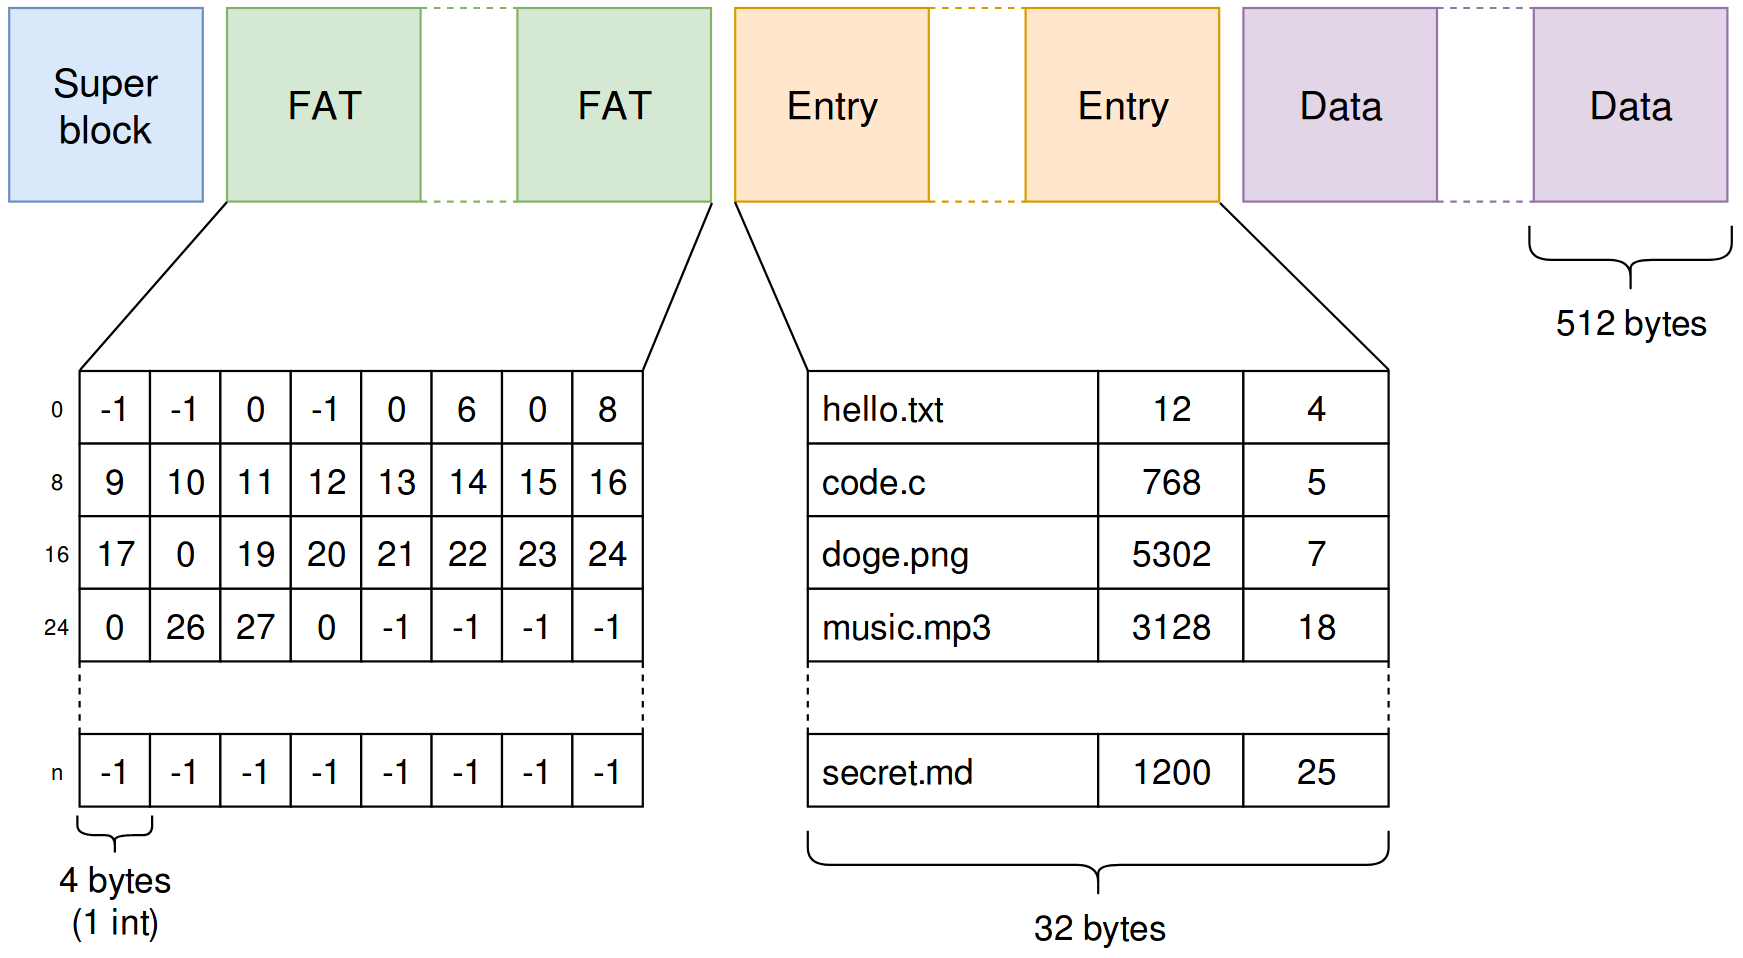
\includegraphics[width=1.0\textwidth]{schema.png}
	\end{center}
\end{figure}

\end{document}
